\section{Interactions of distinct phases of tau with other MAPs}
\label{sec:tau}
\subsection{Tau has one diffusive and one cooperative microtubule binding mode}
\captionsetup[<float-type>]{list=no}
\begin{figure}[b!]
\centering
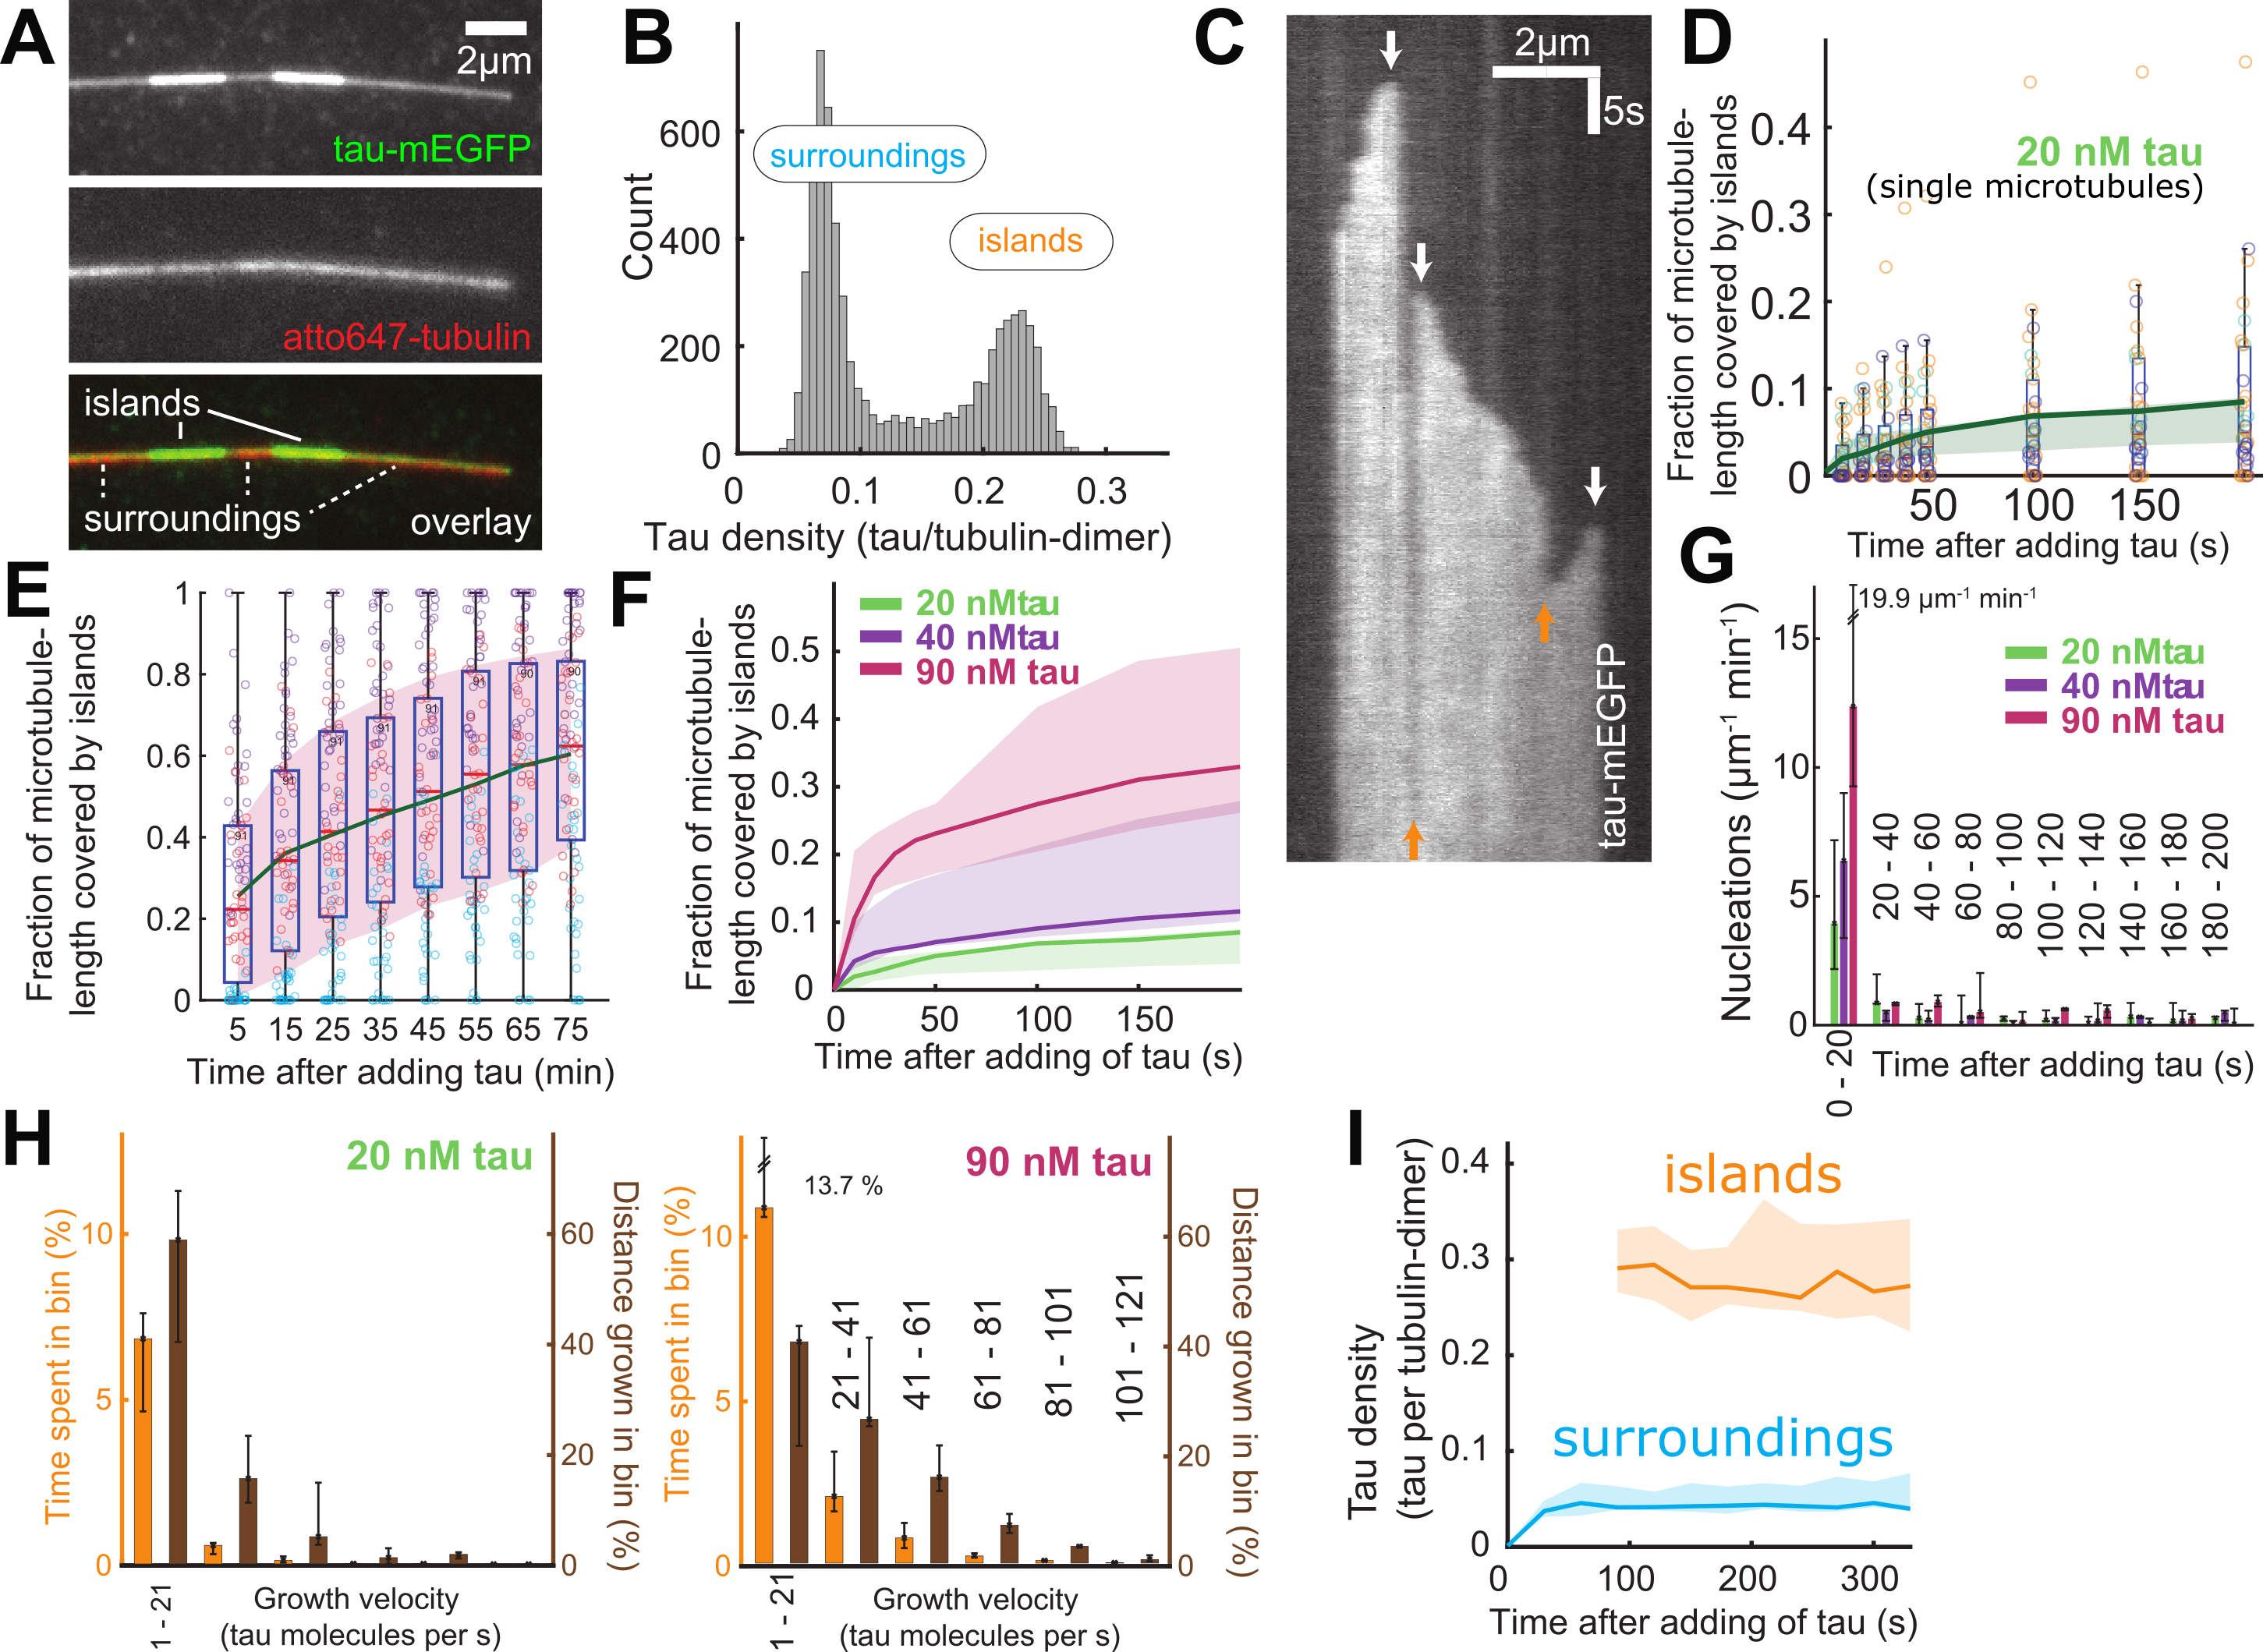
\includegraphics[width=1\linewidth]{Figures/tauGROW.png}
\end{figure}
\captionsetup[<float-type>]{list=yes}
\begin{figure}[t!]
\caption[Tau assembles into tau islands on microtubules.]{\textbf{Tau assembles into tau islands on microtubules.} (A) Multichannel fluorescence micrograph showing areas of high-density tau (bright green) surrounded by regions of low-density tau (dim green) on an Atto-647-labeled microtubule (red). Images taken 5 minutes after adding 20 nM tau. (B) Distribution of fluorescence intensity of tau along the microtubules such as shown in A showing two distinct populations. (C) Kymograph showing the fluorescence signal of tau on a microtubule after the addition 20 nM tau. Initially the microtubule is covered by low tau density. Over time, high-density regions ("islands") start to assemble. White arrows indicate the nucleation points; orange arrows indicate the merging of two neighboring islands growing towards each other. (D) Fraction of microtubule length covered by tau islands at different concentrations after adding tau at time = 0 (n = 3 experiments, shaded area is drawn between the experiment with least coverage and experiment with most coverage, line shows coverage in remaining experiment). Boxplots represent the coverage statistics of individual microtubules. (E) The same data representation as in D, only showing a longer time horizon on the x-axis. (F) Fraction of microtubule length covered by tau islands over time under different tau concentrations (3 experiments per condition). The green line is also shown in D. (G) Tau island nucleation frequency over time (3 experiments per condition, n = 610 nucleation events). Bars show the median; error bars show the minimum and the maximum value. (H) Histograms of island growth velocities at different tau concentrations in solution (n = 2131 velocity traces). The fractions of all bins, together with the fraction of time where growth halted (not shown), add up to 100\%. (I) Exemplary time-trace of the tau density in the islands and their surroundings (Methods) after adding tau (n = 5 microtubules; thick lines and shaded areas indicate median and first and third quartiles, respectively). This experiment was performed with lower frame rate than in C to minimize photo-bleaching. Panels from \cite{Siahaan2019a}.
	}\label{tauGROW}
\end{figure}

To study microtubule-associated tau molecules, we immobilized Atto-647-labeled microtubules on a coverslip, added full-length, human 2N4R (tau441) tau fluorescently labeled on the C-terminus (tau-mEGFP or tau-mCherry) and performed time-lapse imaging using TIRF microscopy (Methods). After the addition of 20 nM tau we observed on the microtubules the formation of high-density tau islands, surrounded by regions with low tau density \pref{tauGROW}{A-C}. These islands, after nucleating from diffraction-limited spots, grew along along a given microtubule to cover more and more of its length \pref{tauGROW}{C,D}. After 75 minutes, most of the microtubule length in a given field of view was covered with islands, with islands still continuing to grow \pref{tauGROW}{E}. When repeating this experiment with higher tau concentrations of 40 and 90nM, microtubules were covered more quickly \pref{tauGROW}{F}, due to a higher nucleation rate of islands \pref{tauGROW}{G} as well as due to faster and more consistent growth at island boundaries \pref{tauGROW}{H}. 

\begin{wrapfigure}{l}{0.6\textwidth}
	\centering
	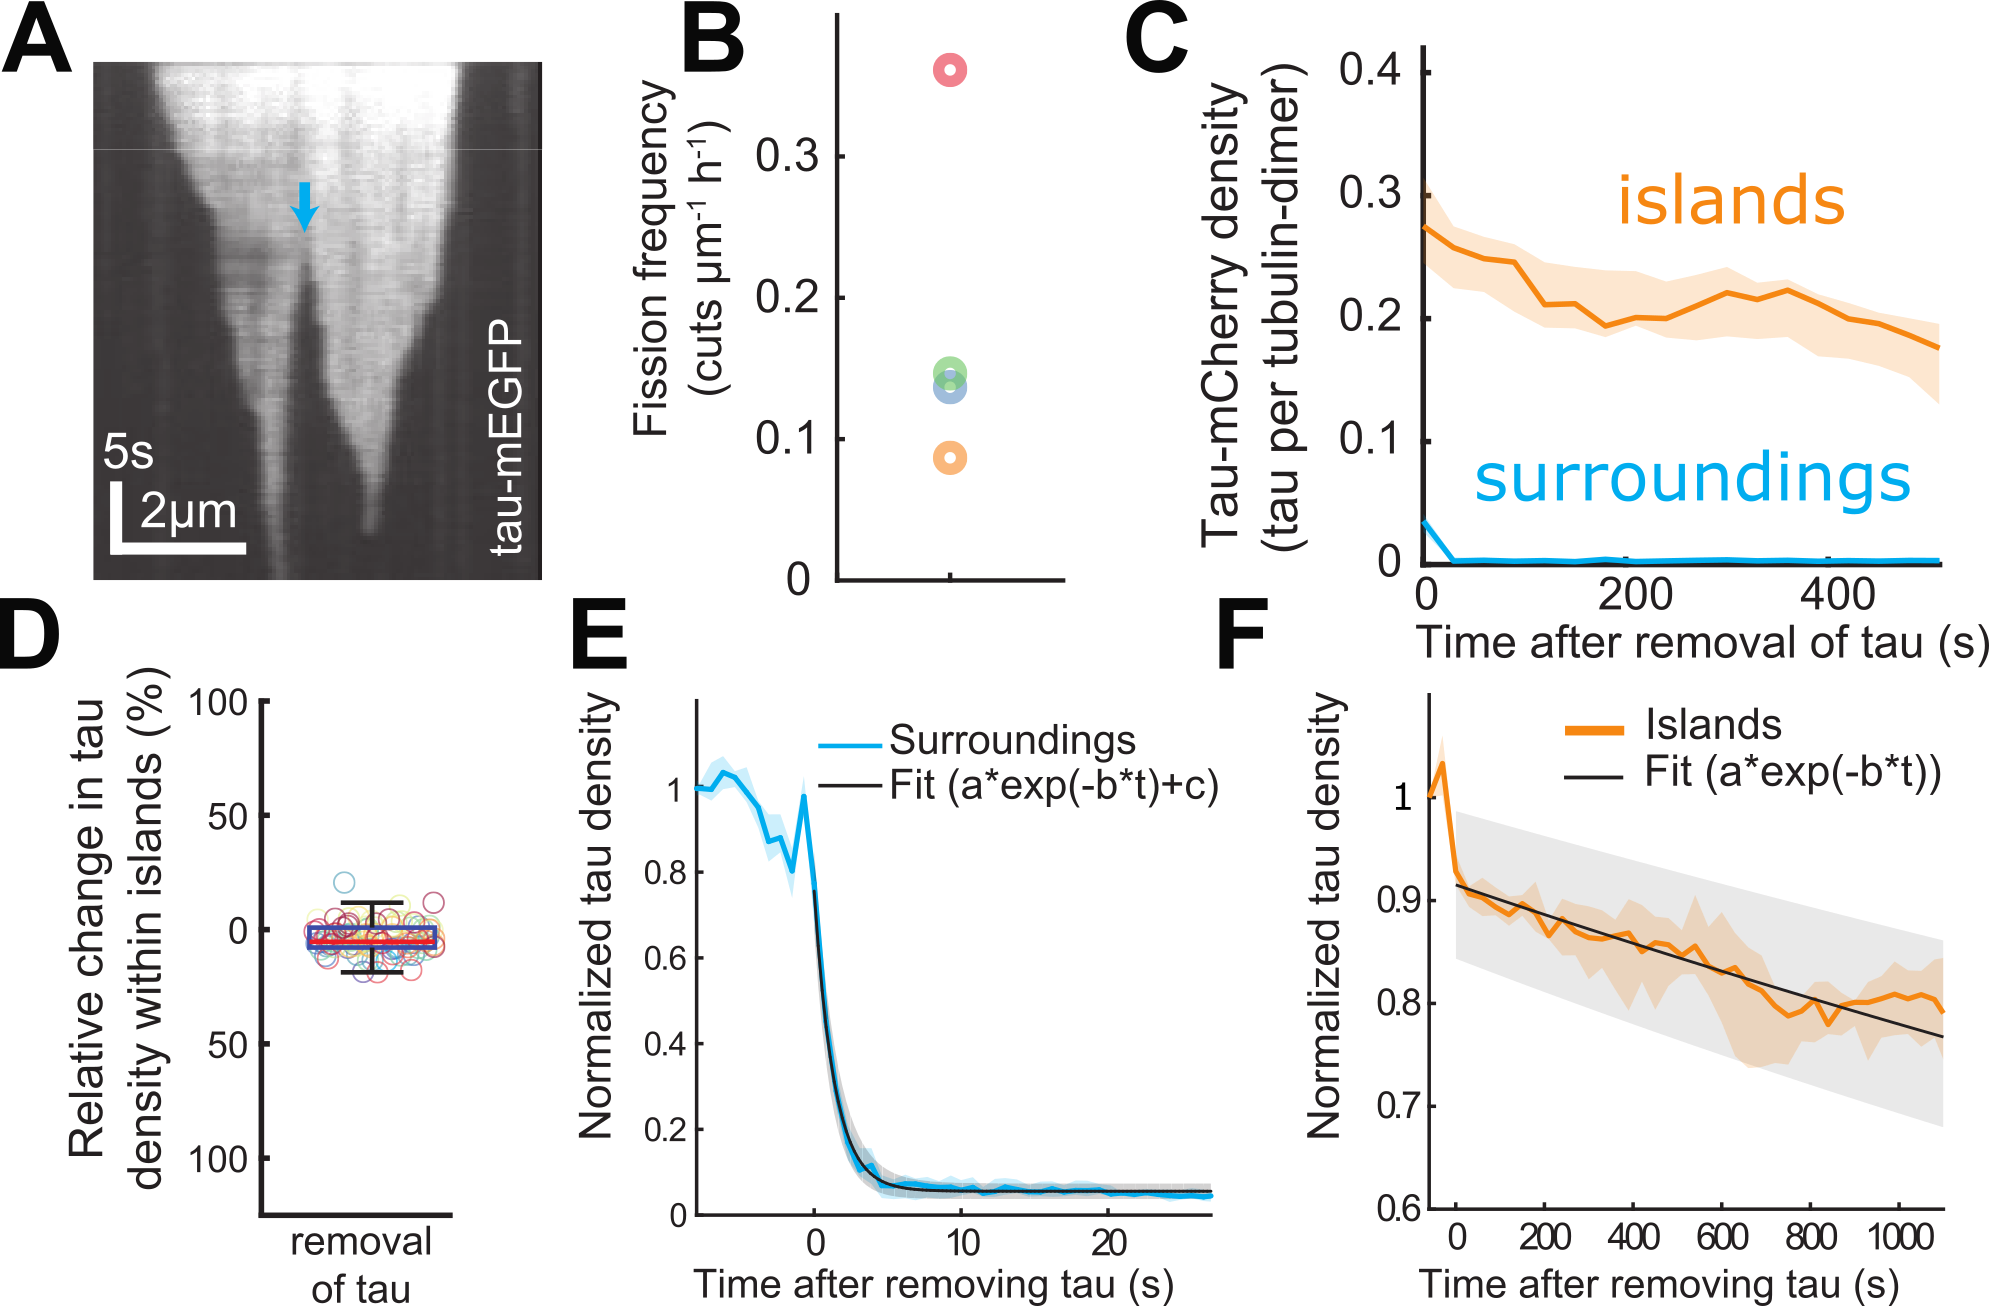
\includegraphics[width=1\linewidth]{Figures/tauSHRINK.png}
	\caption[Tau islands disassemble slowly upon the removal of tau from solution.]{
	\textbf{Tau islands disassemble slowly upon the removal of tau from solution.} (A) Kymograph showing the fluorescence signal of tau on the microtubule after the removal of tau from solution. The blue arrow indicates a fission event that here occurred during island disassembly. (B) Frequency of fissions occurring within islands upon removing tau from solution. Colors encode different experiments. (C) Distribution of island disassembly velocities upon removing tau from solution. Colors encode experiments (same as in B), circles represent deassembly traces. (D) Exemplary time-trace of the tau density inside and outside the islands after removing (20nM) tau from solution (n = 9 microtubules). (E,F) Exemplary time-trace of tau density inside and tau density outside the islands after removing (20nM) tau from solution, analogous to the results presented in E (n = 6 microtubules). Single exponential fits are indicated by solid lines. This experiment had been repeated 4 and 3 times for islands and surroundings, respectively, with similar results. In time-traces, thick lines and shaded areas indicate median and first and third quartiles, respectively. Panels from \cite{Siahaan2019a}.
		}\label{tauSHRINK}
\end{wrapfigure}
Generally, the islands did not grow monotonously at their boundaries, but with variable velocities in the order of 25 nm/s, corresponding to about 10 molecules added per second \pref{tauGROW}{H}. Importantly, the tau density in the islands stayed constant during the period of growth \pref{tauGROW}{I}, suggesting that the islands grow by the addition of tau molecules at their boundaries, reminiscent of epitaxial growth of thin films. As another indication that islands are formed by a well-defined tau layer occupying the entire accessible surface of the microtubule, we never observed an increase in the tau density when the boundaries of neighboring growing islands came into contact \pref{tauGROW}{C}.\par

When tau was removed from solution, the islands disassembled slowly from their boundaries, occassionally fissioning inside \pref{tauSHRINK}{A-B}. In contrast to island growth, this island shrinkage rarely halted \pref{tauSHRINK}{B}, and proceeded with a median velocity of approximately 2 tau molecules unbinding per second at a given island boundary \pref{tauSHRINK}{C}. Importantly, the tau density within islands only declined very slowly after removing tau from solution compared to the decline in tau density on all regions outside of islands (the “island surroundings”) \pref{tauSHRINK}{D}. Indeed, while in the surroundings tau unbound with a time constant of about 2 seconds as inferred from the decay of the fluorescence signal \pref{tauSHRINK}{E}, within the islands tau molecules unbound on the timescale of tens of minutes \pref{tauSHRINK}{F}. This extremely low unbinding rate explains the preservation of the islands in absence of tau in solution and suggests that the occasional island fissions observed during disassembly occur after rare events of tau molecules unbinding from inside the island. The large difference in the tau unbinding rates within islands compared to island surroundings, together with the assembly and disassembly kinetics at the island boundaries, indicate that tau molecules in the islands bind to microtubules cooperatively. 

\begin{figure}[h]
\centering
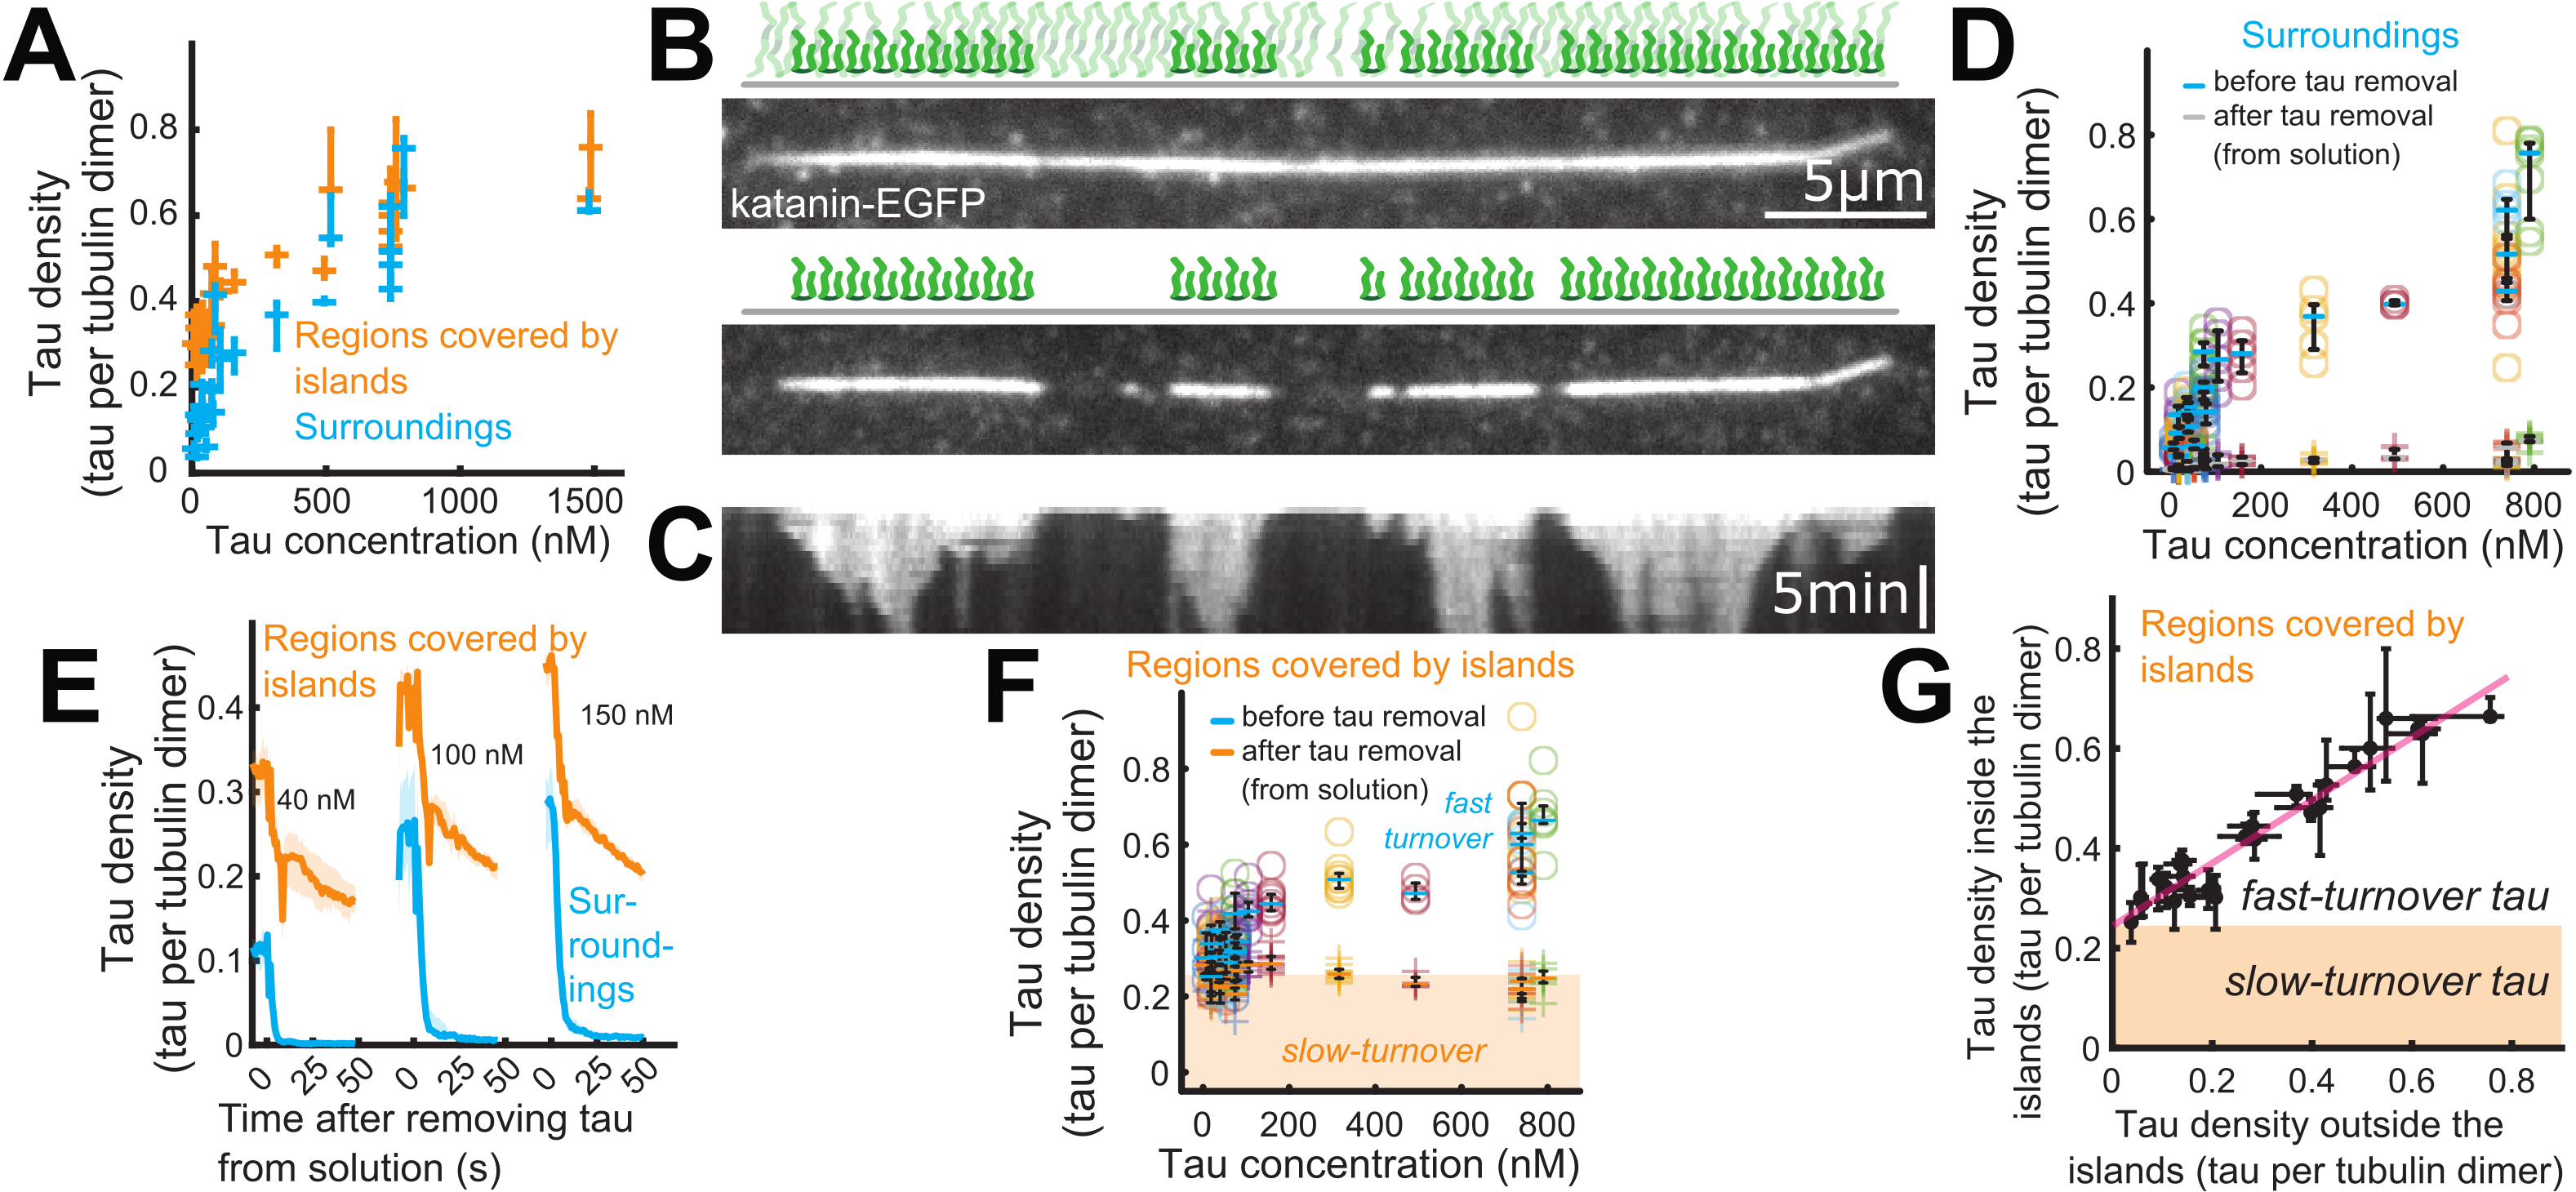
\includegraphics[width=1\linewidth]{Figures/tau_flushouts.png}
\caption[Tau islands are distinguished by cooperative tau binding.]{
\textbf{Tau islands are distinguished by cooperative tau binding} (A) The (equilibrium) density of tau on microtubules plotted against concentration of tau in solution. Horizontal lines indicate the three quartiles. (B) Fluorescence micrographs showing the coverage of a microtubule by tau. Upper panel: 5 minutes after the addition of 0.8 µM tau. Lower panel: 30 seconds after the removal of tau from solution. (C) Kymograph of the experiment presented in B showing the disassembly of the islands after removing tau from solution. (D) Tau densities in microtubule regions surrounding islands, before and after removing tau from solution. (E) Exemplary time-traces of tau density outside and inside the islands during subsequent cycles of adding increasing concentrations of tau followed by removing tau from solution. Experiment such as presented in D and F. (F) Tau densities in microtubule regions with islands, before and after removing tau from solution. (G) The (equilibrium) density of tau on microtubules inside island regions plotted against the density of tau in the surroundings, using the data presented in A. The red line visualizes a linear fit. Points are color-coded by experiment, horizontal lines indicate the three quartiles of each experiment (in some panels the median is indicated by circle). In C and G, the characteristic island density (Main text, Methods) is indicated by the height of the shaded area. Panels from \cite{Siahaan2019a}.
	}\label{tauflushouts}
\end{figure}

To more thoroughly explore whether and how the phenomena we observed were concentration-dependent, we conducted additional experiments, increasing the range of tested tau concentrations. Our observations revealed that island formation did not occur below a critical tau concentration of approximately 5 nM (n = 245 microtubules in 5 experiments; these experiments were performed by my colleague Valerie Siahaan). Above this threshold, we noted that the tau density both within and outside the islands increased with the tau concentration in solution \pref{tauflushouts}{A}. We had noticed this previously already with our experiments at 20, 40 and 90nM tau, yet with much larger concentrations it in addition became apparent that tau binding to microtubules in our buffer condition reaches a saturation point at around 1000nM \pref{tauflushouts}{A}. Moreover,under such saturated binding conditions, the density on the microtubule appears to be uniform \pref{tauflushouts}{A}, i.e., a distinction between islands and surroundings based on tau density can no longer be made. However, upon removing tau from solution, in areas surrounding the islands, the tau density rapidly returned to background levels within seconds \pref{tauflushouts}{B-E}, consistent with our previous surrounding-related findings when removing 20nM Ase1 \pref{tauSHRINK}{E}. Meanwhile, the islands persisted \pref{tauflushouts}{B-C} as observed previously \pref{tauSHRINK}{A}. However, at higher Ase1 concentrations it became apparent that the tau density within the islands exhibits a two-phase decay upon removal of tau: an initial rapid, uniform decrease along the entire island length, followed by a slower density reduction \pref{tauflushouts}{E}. Importantly, the tau density within the islands, following the rapid density drop, consistently measured 0.26 ± 0.05 tau molecules per tubulin dimer (average ± SD, n = 101 microtubules, 14 experiments, Methods). This value remained constant regardless of the initial tau concentration in solution \pref{tauflushouts}{F}. \par

Combining these results with our findings from \aref{tauGROW}{} and \aref{tauSHRINK}{}, we conclude that cohesive islands on microtubules form through the cooperative binding of tau molecules, resulting in their slow unbinding. At physiological tau concentrations \parencite{Wegmann}, ranging from 0.5 to 1.5 µM, we observed the co-localization of rapidly turning over tau molecules with the islands. The density of these co-localized tau molecules, which appears to correlate with the tau concentration in solution similarly to the tau density outside the islands \pref{tauflushouts}{G}, does not seem to be part of the cooperative island formation process. \par

\begin{figure}[h!]
	\centering
	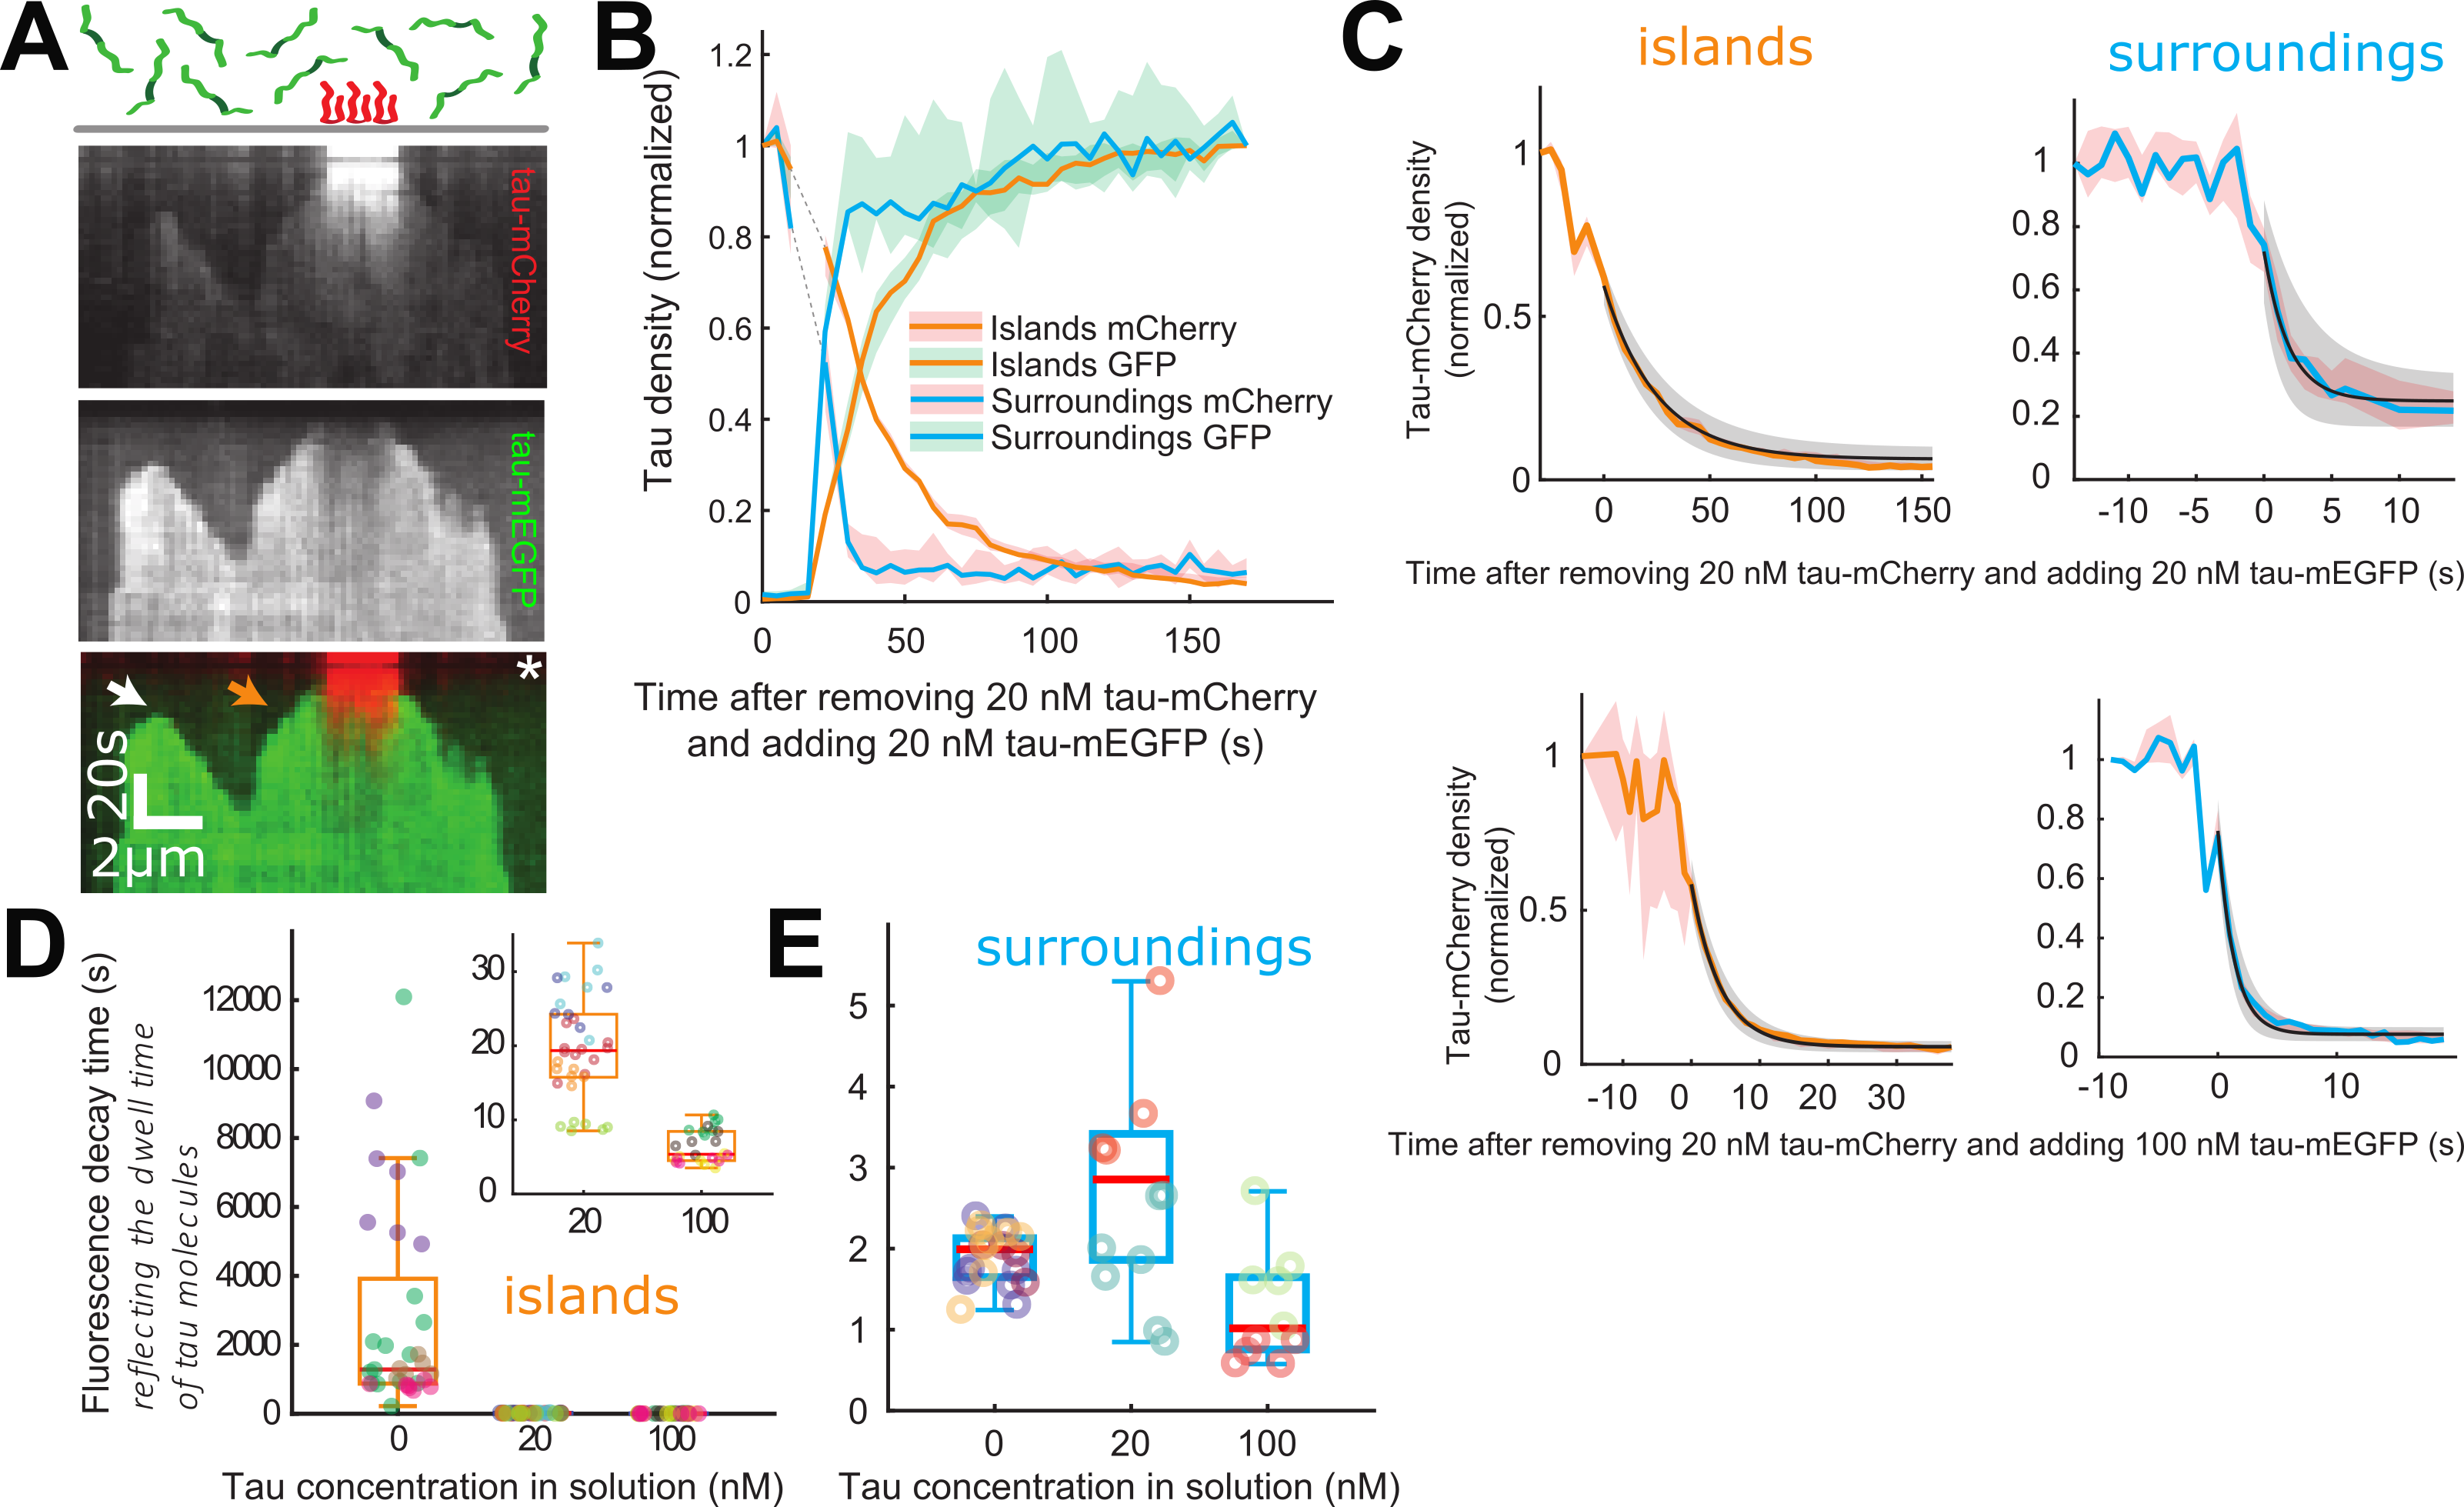
\includegraphics[width=1\linewidth]{Figures/tau_EXCHANGE.png}
	\caption[Tau molecules in the islands exchange with tau in solution.]{
	\textbf{Tau molecules in the islands exchange with tau in solution.} (A) Multichannel kymograph showing an island pre-formed in presence of 20 nM tau-mCherry (red). After the addition (time marked by white asterisk) of 20 nM tau-mEGFP (green), removing most of the tau-mCherry from solution, tau-mEGFP replaces tau-mCherry inside and outside of the islands. An example of an island resuming its growth by the addition of tau-mEGFP is marked by an orange arrow, a nucleation event is marked by a white arrow. (B) Exemplary time-trace of normalized tau-mCherry and tau-mEGFP density inside and outside the islands after exchange of 20 nM tau-mCherry for 20 nM tau-mEGFP. Photo-bleaching during this experiment was negligible (Methods); the dotted line indicates that the sample was out of focus at the time. (D) Dwell times of tau-mCherry derived from fitting exponential decay functions to tau densities over time in the surroundings of islands. (E) Same representation as D, for island regions. The inset displays the 20 nM and 100 nM boxes on a magnified y-scale. Data points are color-coded by experiments. Panels from \cite{Siahaan2019a}.
		}\label{tauexchange}
\end{figure}

To further explore the dynamics of tau molecules in the islands, we formed islands using 20 nM tau-mCherry and, after 15 minutes, replaced the assay buffer by a solution containing 20 nM tau-mEGFP. Outside the islands, tau-mCherry was replaced quickly by tau-mEGFP \pref{tauexchange}{A}. This included the growth of new islands, which now proceeded by addition of tau-mEGFP \pref{tauexchange}{A}. However, within the islands, tau-mCherry visibly remained bound to microtubules for longer \pref{tauexchange}{A,B}. We quantified this effect by fitting the tau density in a given region at different time points to an exponential decay function \pref{tauexchange}{C}: In the low-density regions, surrounding the islands, tau-mCherry dissociated from the microtubules with an average residence time of about 3 seconds \pref{tauexchange}{D}, a value comparable to the residence time where tau was completely removed from solution without replacement \pref{tauSHRINK}{E}. By contrast, within the islands tau-mCherry dissociated markedly slower, with an average residence time of 20 ± 7 s (average ± SD) seconds \pref{tauexchange}{E}. This value is, however, substantially faster than in the situation when tau was completely removed from solution, in which case the dwell time was 45 ± 46 min (compare to \aref{tauSHRINK}{F}). Thus, we observed that tau unbinding from the islands depends on the tau concentration in solution. As another piece of evidence confirming this dependence, we observed that tau-mCherry unbound form islands even faster when adding 100nM tau-mEGFP as compared to the addition of 20nM tau-mEGFP (in this case, the dwell time was 6.4 ± 2.1 s) \pref{tauexchange}{E}.\par

\begin{wrapfigure}{l}{0.5\textwidth}
	\centering
	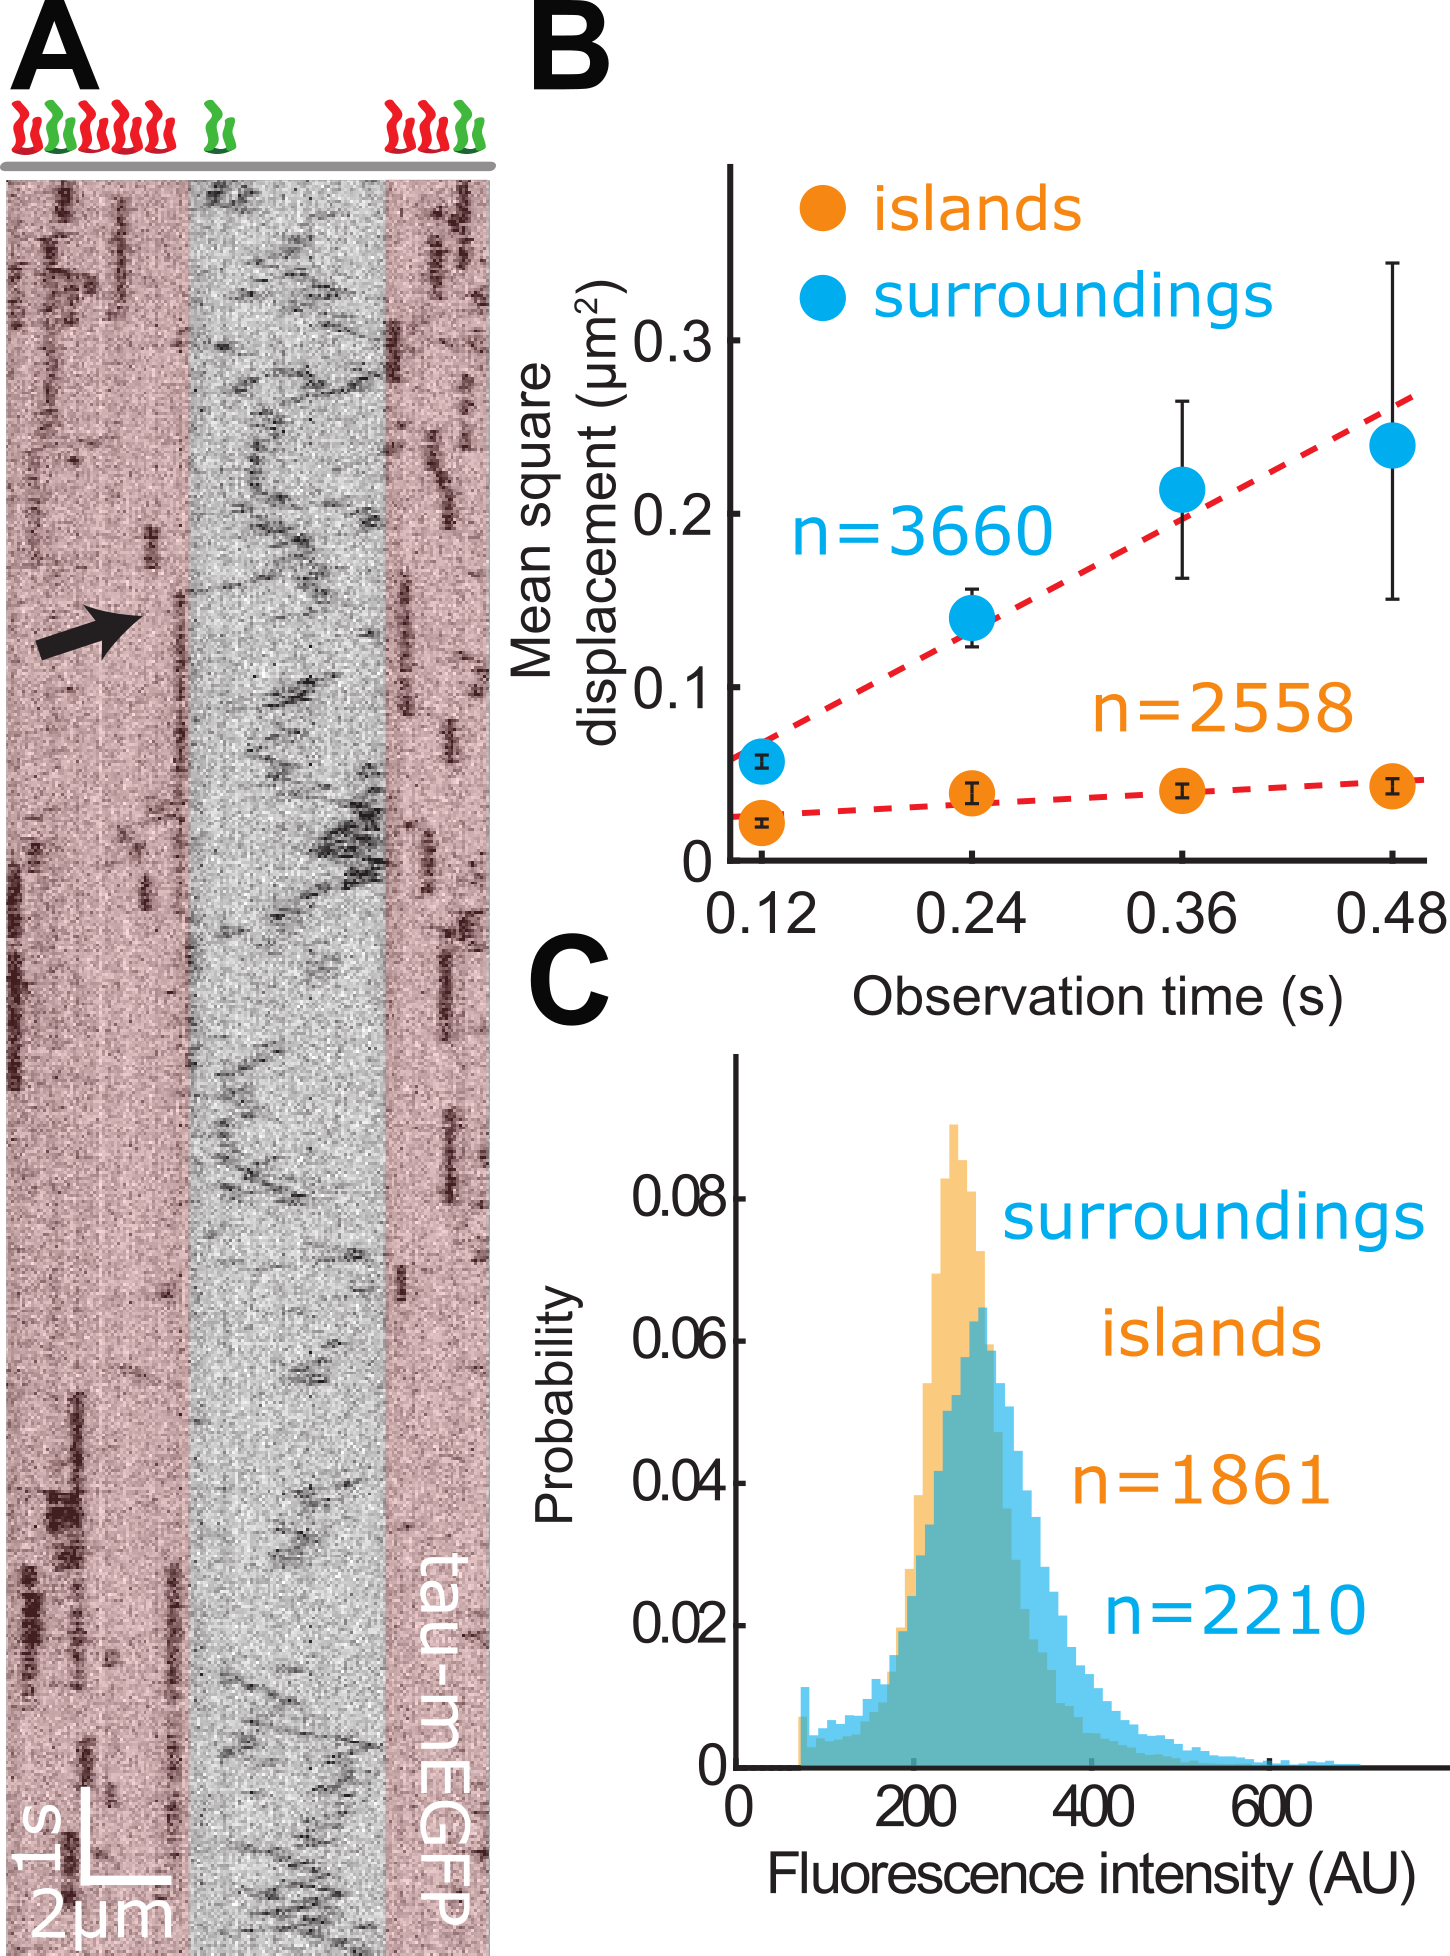
\includegraphics[width=1\linewidth]{Figures/tau_singleMolecules.png}
	\caption[Tau molecules are stationary within the islands.]{
	\textbf{Tau molecules are stationary within the islands.} (A) Intensity-inverted kymograph showing single tau-mEGFP molecules interacting with a microtubule covered by two tau-mCherry islands (20nM tau-mCherry in solution). Outside the islands (light grey region), tau-mEGFP diffuses rapidly, whereas inside the islands (light red regions), tau-mEGFP is bound stationarily. An event where a diffusing tau-mEGFP molecule gets associated with an island is indicated with a black arrow. (B) Mean square displacement over time of single tau-EGFP molecules inside and outside tau-mCherry islands. (C) Histograms of fluorescence intensities of single tau-mEGFP particles bound to microtubules in experiments as presented in A, showing that tau-mEGFP is associated with the microtubule in monomeric form. (D) Intensity-inverted kymograph showing single tau-mEGFP molecules interacting with a microtubule covered by a tau-mCherry island (100nM tau-mCherry in solution). The orange arrow points toward an example of a brief and diffusive interaction of a tau molecules inside the island. The blue arrows indicate events where an island-bound tau molecule appear to briefly change their binding mode and diffuse along the microtubule. Much more than in A, we here also observed very brief tau interactions within islands (white arrow points to an example). Panels from \cite{Siahaan2019a}, except for panel D, which is published only in this thesis (experiment conducted by Valerie Siahaan, data analyzed and interpreted by me).
		}\label{tausingle}
\end{wrapfigure}
To further study the spatio-temporal interaction dynamics of tau and microtubules, we formed islands using a mixture of 20 nM tau-mCherry and 1 nM tau-mEGFP. This strategy allowed us to observe the motion of individual tau-mEGFP molecules even within tau islands, as these islands were mainly comprised of tau-mCherry molecules. In the low-density regions, single tau-mEGFP molecules diffused rapidly \pref{tausingle}{A}. By contrast, in the islands the tau-mEGFP molecules did not display any noticable movement \pref{tausingle}{A}. Occasionally, single tau-mEGFP molecules initially diffusing outside an island became stationary when associating with an island boundary \pref{tausingle}{A}. Quantifying these phenomena (Methods), we measured that outside the islands, tau molecules diffused with a diffusion constant of 0.27 ± 0.15 $\mu m^2s^{-1}$ (95\% confidence bounds) \pref{tausingle}{B}, comparable to values reported before by \cite{Hinrichs2012b}. Within the islands, we measured tau-mEGFP molecules to have a diffusion constant of 0.027 ± 0.016 $\mu m^2s^{-1}$ \pref{tausingle}{B}. To test whether we indeed observed single tau molecules rather than conglomerates which had formed in solution, we generated fluorescence intensity histogram of individual tau-mEGFP particles \pref{tausingle}{C}. These exhibited a single Gaussian profile in the islands just as in their surroundings, indicating that tau-tau interactions indeed occurred only on the microtubule lattice. Finally, we formed islands using a mixture of 100 nM tau-mCherry and 1 nM tau-mEGFP. Consistent with the results shown in \aref{tauflushouts}{}, we observed diffusive and/or brief interactions of tau molecules inside islands \pref{tausingle}{D}.\par

\begin{figure}[h!]
	\centering
	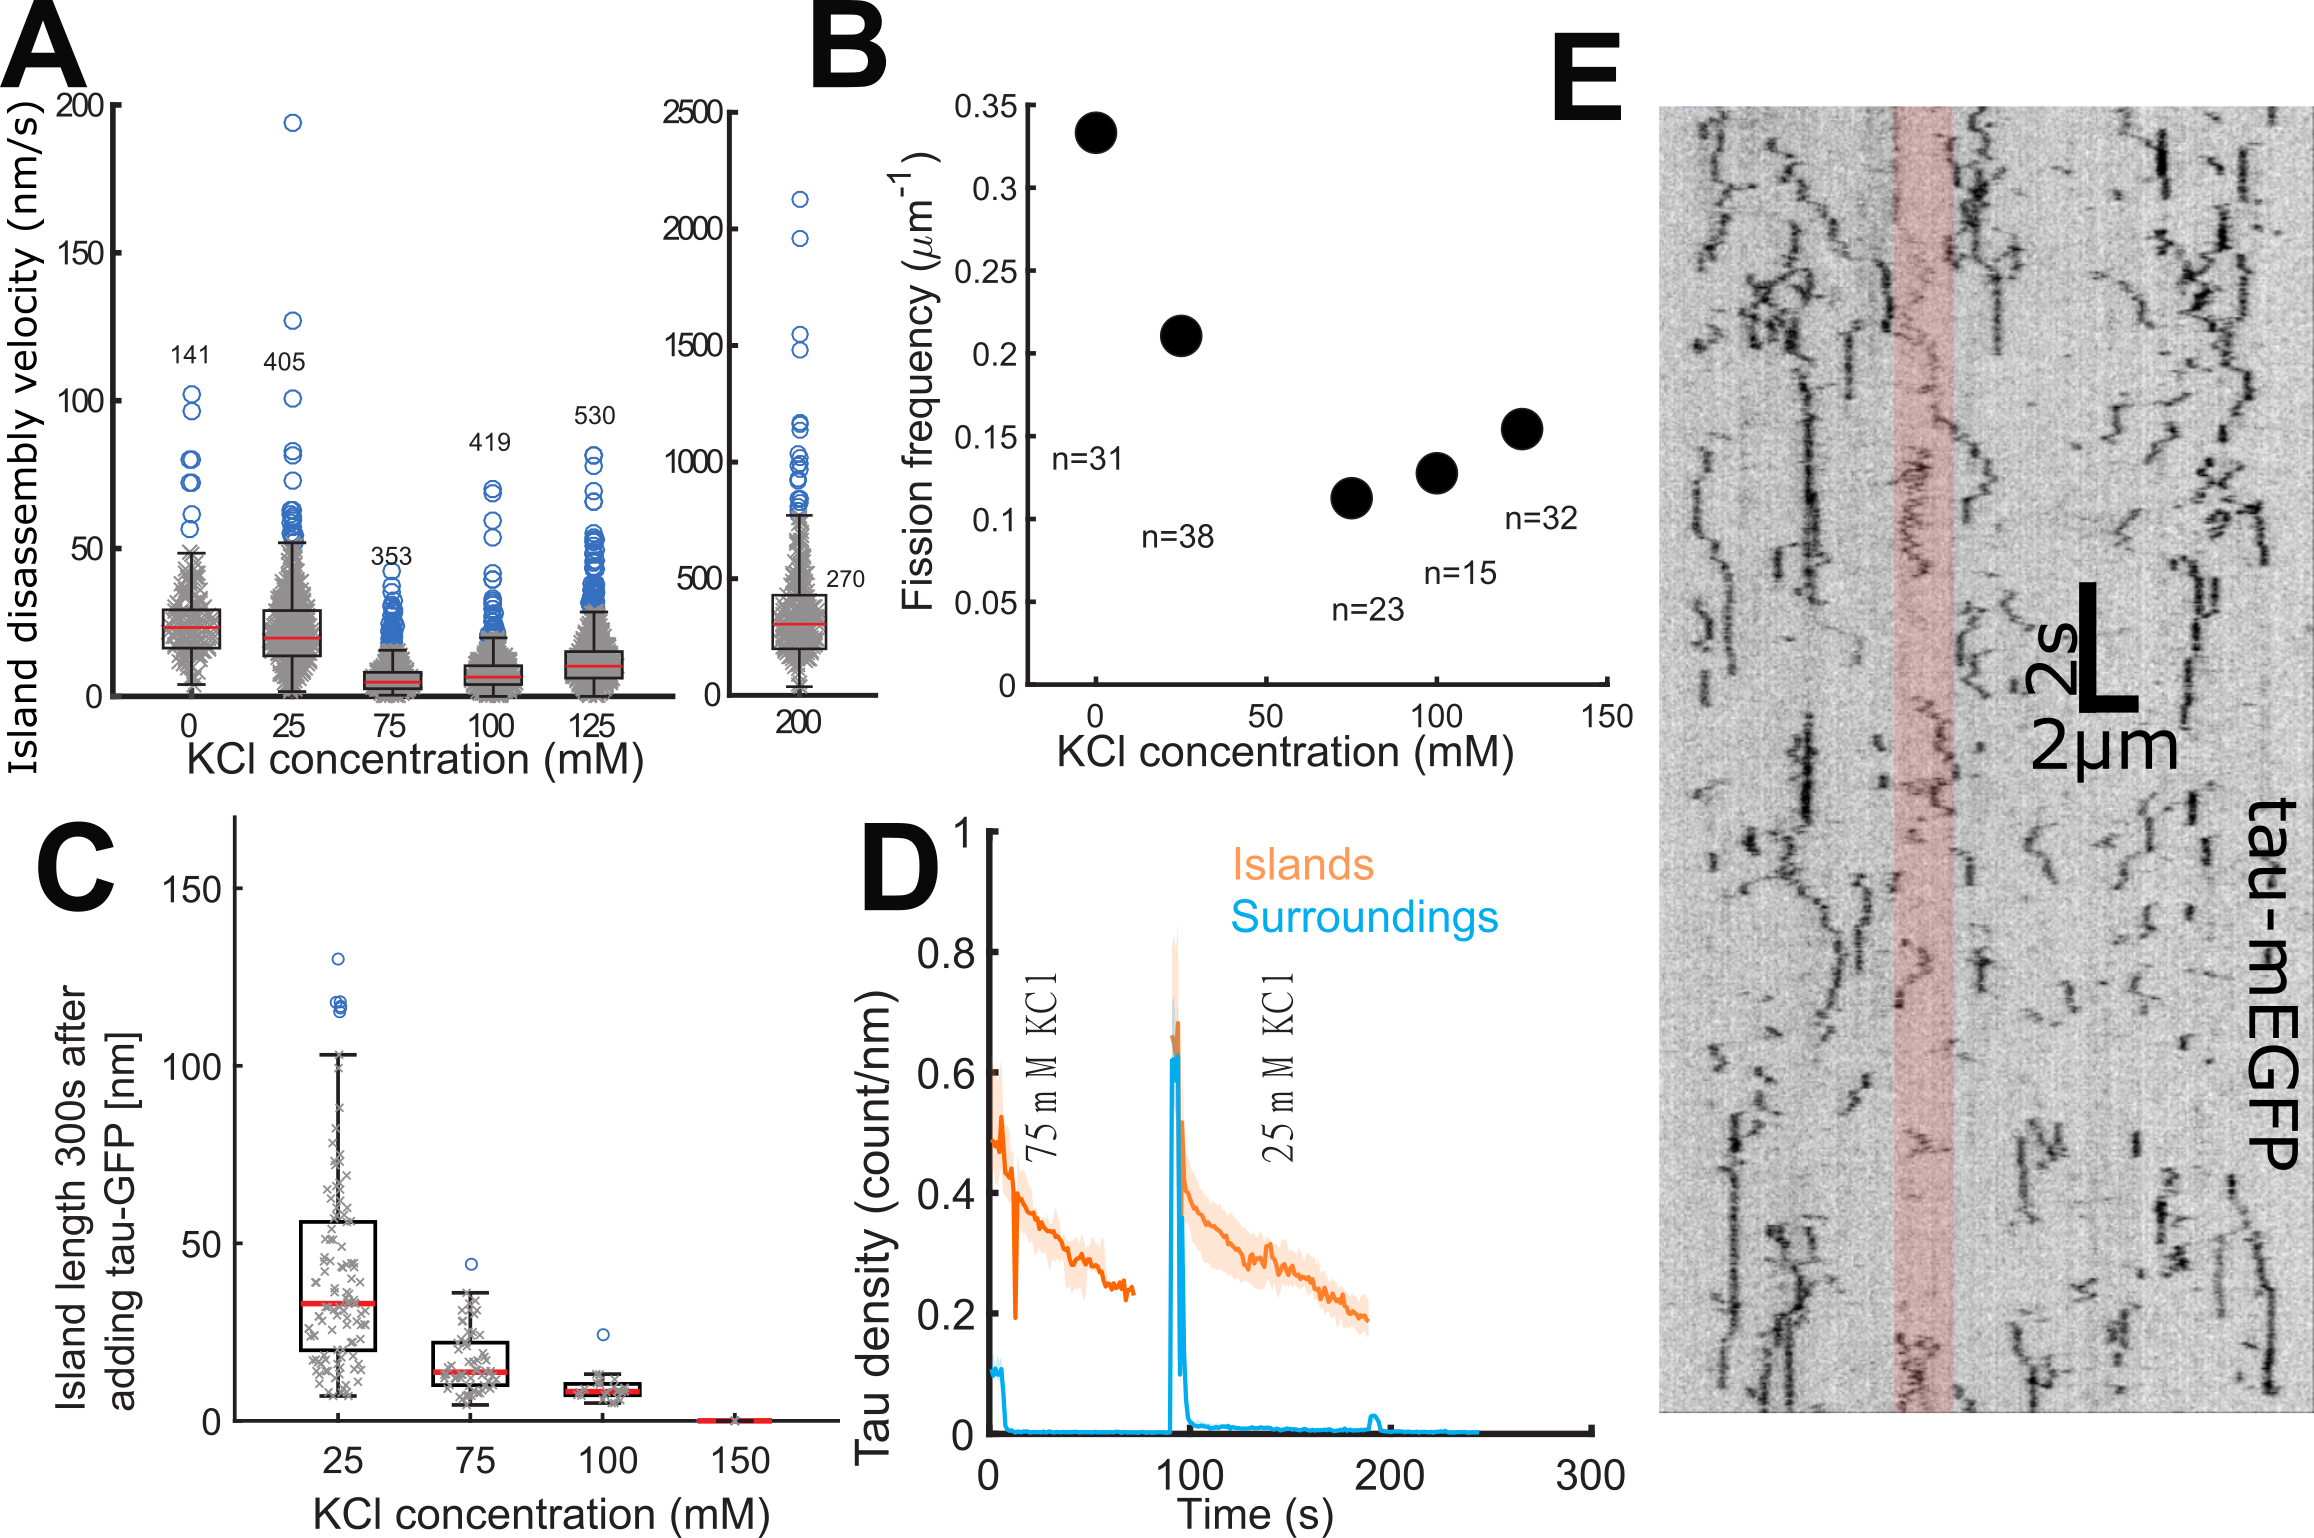
\includegraphics[width=1\linewidth]{Figures/tausalt.png}
	\caption[The preferred binding mode of tau varies with ionic strength.]{
	\textbf{The preferred binding mode of tau varies with ionic strength.} (A,B) Island disassembly velocities and fission frequencies at different concentrations of KCl (after tau had been removed from solution; islands had been grown at 75mM KCl). Numbers show the number of measured disassembly periods (panel A) or observed fissions (panel B). (C) Lengths of islands measured 300s after adding 40nM tau at varying concentrations of KCl. (D) Cycles of adding and removing 100nM tau to/from solution (additions at t=-100s and t=100s, removals roughly at t=10s and t=110s). In the second cycle, the solution contained only 25mM KCl rather than 75mM, which was used in all previously shown experiments. Bleaching was not negligible in this experiment. (E) Intensity-inverted kymograph showing single tau-mEGFP molecules interacting with a microtubule covered by a tau-mCherry island (highlighted by the red area) at 25mM KCl. Findings shown in this figure have not been published yet.
		}\label{tausalt}
\end{figure}

Finally, we were interested in exploring some plausible determinants of island assembly beside tau concentration. First, because the N-terminus of tau mediates tau-tau interactions \parencite{Gamblin2003}, we attempted to grow tau islands with a truncated tau construct comprising the four-repeat microtubule-binding domain and the C-terminus but lacking the N-terminus (tau$\Delta$N-mEGFP, \aref{tauconstructs}{}). Although tau$\Delta$N-mEGFP did interact with the microtubules, we did not observe any island formation even at 0.5 µM tau$\Delta$N-mEGFP (these experiments were performed by my colleague Valerie Siahaan). Second, we varied the ionic strength of our buffer solution by varying the concentration of KCl (these experiments were largely performed by me; for reasons of space we did not include these findings in \cite{Siahaan2019a}). We noticed that increasing as well as decreasing the concentration of KCl from the level we had used for the experiments we have reported on so far, namely 75mM, both tended to decrease the stability of tau islands: 0, 25, 100, and 125nM KCl islands disassembled quicker once tau was removed from solution than at 75mM KCl \pref{tausalt}{A,B}. Disassembly speed was drastically higher at 200mM KCl \pref{tausalt}{A right panel}. Generally, tau binding to the microtubule was less pronounced at higher KCl concentrations, both in terms of island formation and binding to surrounding regions (data not shown). However, interestingly, at 0 and 25mM KCl, island assembly was more pronounced than at 75mM KCl \pref{tausalt}{C}. At the same time, at these low KCl concentrations, more tau bound to the microtubule via the diffusive binding mode, visible from the high tau densities in the surrounding regions \pref{tausalt}{D}. Consistent with the observation that islands at lower ionic strengths were less stable, when looking at single tau-mEGFP molecules in a tau-mCherry-dominated environment, we observed that the distinction between binding within the islands versus binding outside the islands was less clear-cut than at 75mM KCl \pref{tausalt}{E}. Tau molecules appeared to switch regularly between diffusive and stationary interactions within islands, though the diffusive interactions appeared more tightly bound to the microtubule than outside the islands \pref{tausalt}{E}. We had observed such switches already at 75mM KCl, though at that condition these switches were much less prevalent \pref{tausingle}{D}.\par

Combined, our results show that tau molecules bind to microtubules in two distinct binding modes. The diffusive binding mode had already been described before \parencite{Hinrichs2012b}. However, we together with \cite{tan2019microtubules} discovered another, cooperative, binding mode, which results in the formation of what we termed tau islands (in more recent publications on the topic the term "envelopes" is used, see e.g. \cite{siahaan2022microtubule}). This cooperative binding mode, unlike the diffusive mode, is dependent on the N-terminus region of tau. The strength of this cooperative binding mode moreover varies differently with ionic strength than the strength of the diffusive binding mode.